\chapter{Introduction}
\label{chp:intro}

This is the introduction to your work. Explain the overarching 
research area where this falls under, and motivate your project.

\section{\LaTeX{} tips \& tricks}

Look at the source code for this section to see the \LaTeX{} source
for what follows.

This is a reference~\cite{turing1937}. They are included in file \texttt{references.bib}. Note that the \texttt{hyperref} package has added a link there for you. If you click on it, this should take you to the corresponding reference in the Bibliography section. Don't worry about the strange frame around it, it does not show when printed (and some pdf viewers are not really good at rendering it -- that includes Overleaf).

You can leave comments in little boxes like this. This is very useful when collaborating. Your advisor can use it to leave notes in your document.\note{This is useful.}

Some environments are already predefined for you.

\begin{example}
An example \emph{example}.
\end{example}

\begin{remark}
An unremarkable \emph{remark}.
\end{remark}

\begin{definition}
A definitive \emph{definition}.
\end{definition}

\begin{lemma}
\label{lmm:helper}
A \emph{helper} theorem.
\end{lemma}

\begin{theorem}
\label{thm:result}
A \emph{theorem}.
\end{theorem}

\begin{proof}
A proof of Theorem~\ref{thm:result} using Lemma~\ref{lmm:helper}.
\end{proof}

\begin{corollary}
A \emph{consequence} of Theorem~\ref{thm:result}
\end{corollary}

If you need to define other environments as above, they are in the
file \texttt{configs/preamble.tex}.

You can include macros and definitions in \texttt{configs/newcommands.tex} to make typing easier and keep consistency throughout the document. For example: \pyth{a}{b}{c}.

The \texttt{graphicx} package allows you to include pictures like the Von Neumann Architecture in Figure~\ref{fig:von_neumann_arch}.

\begin{figure}
    \centering
    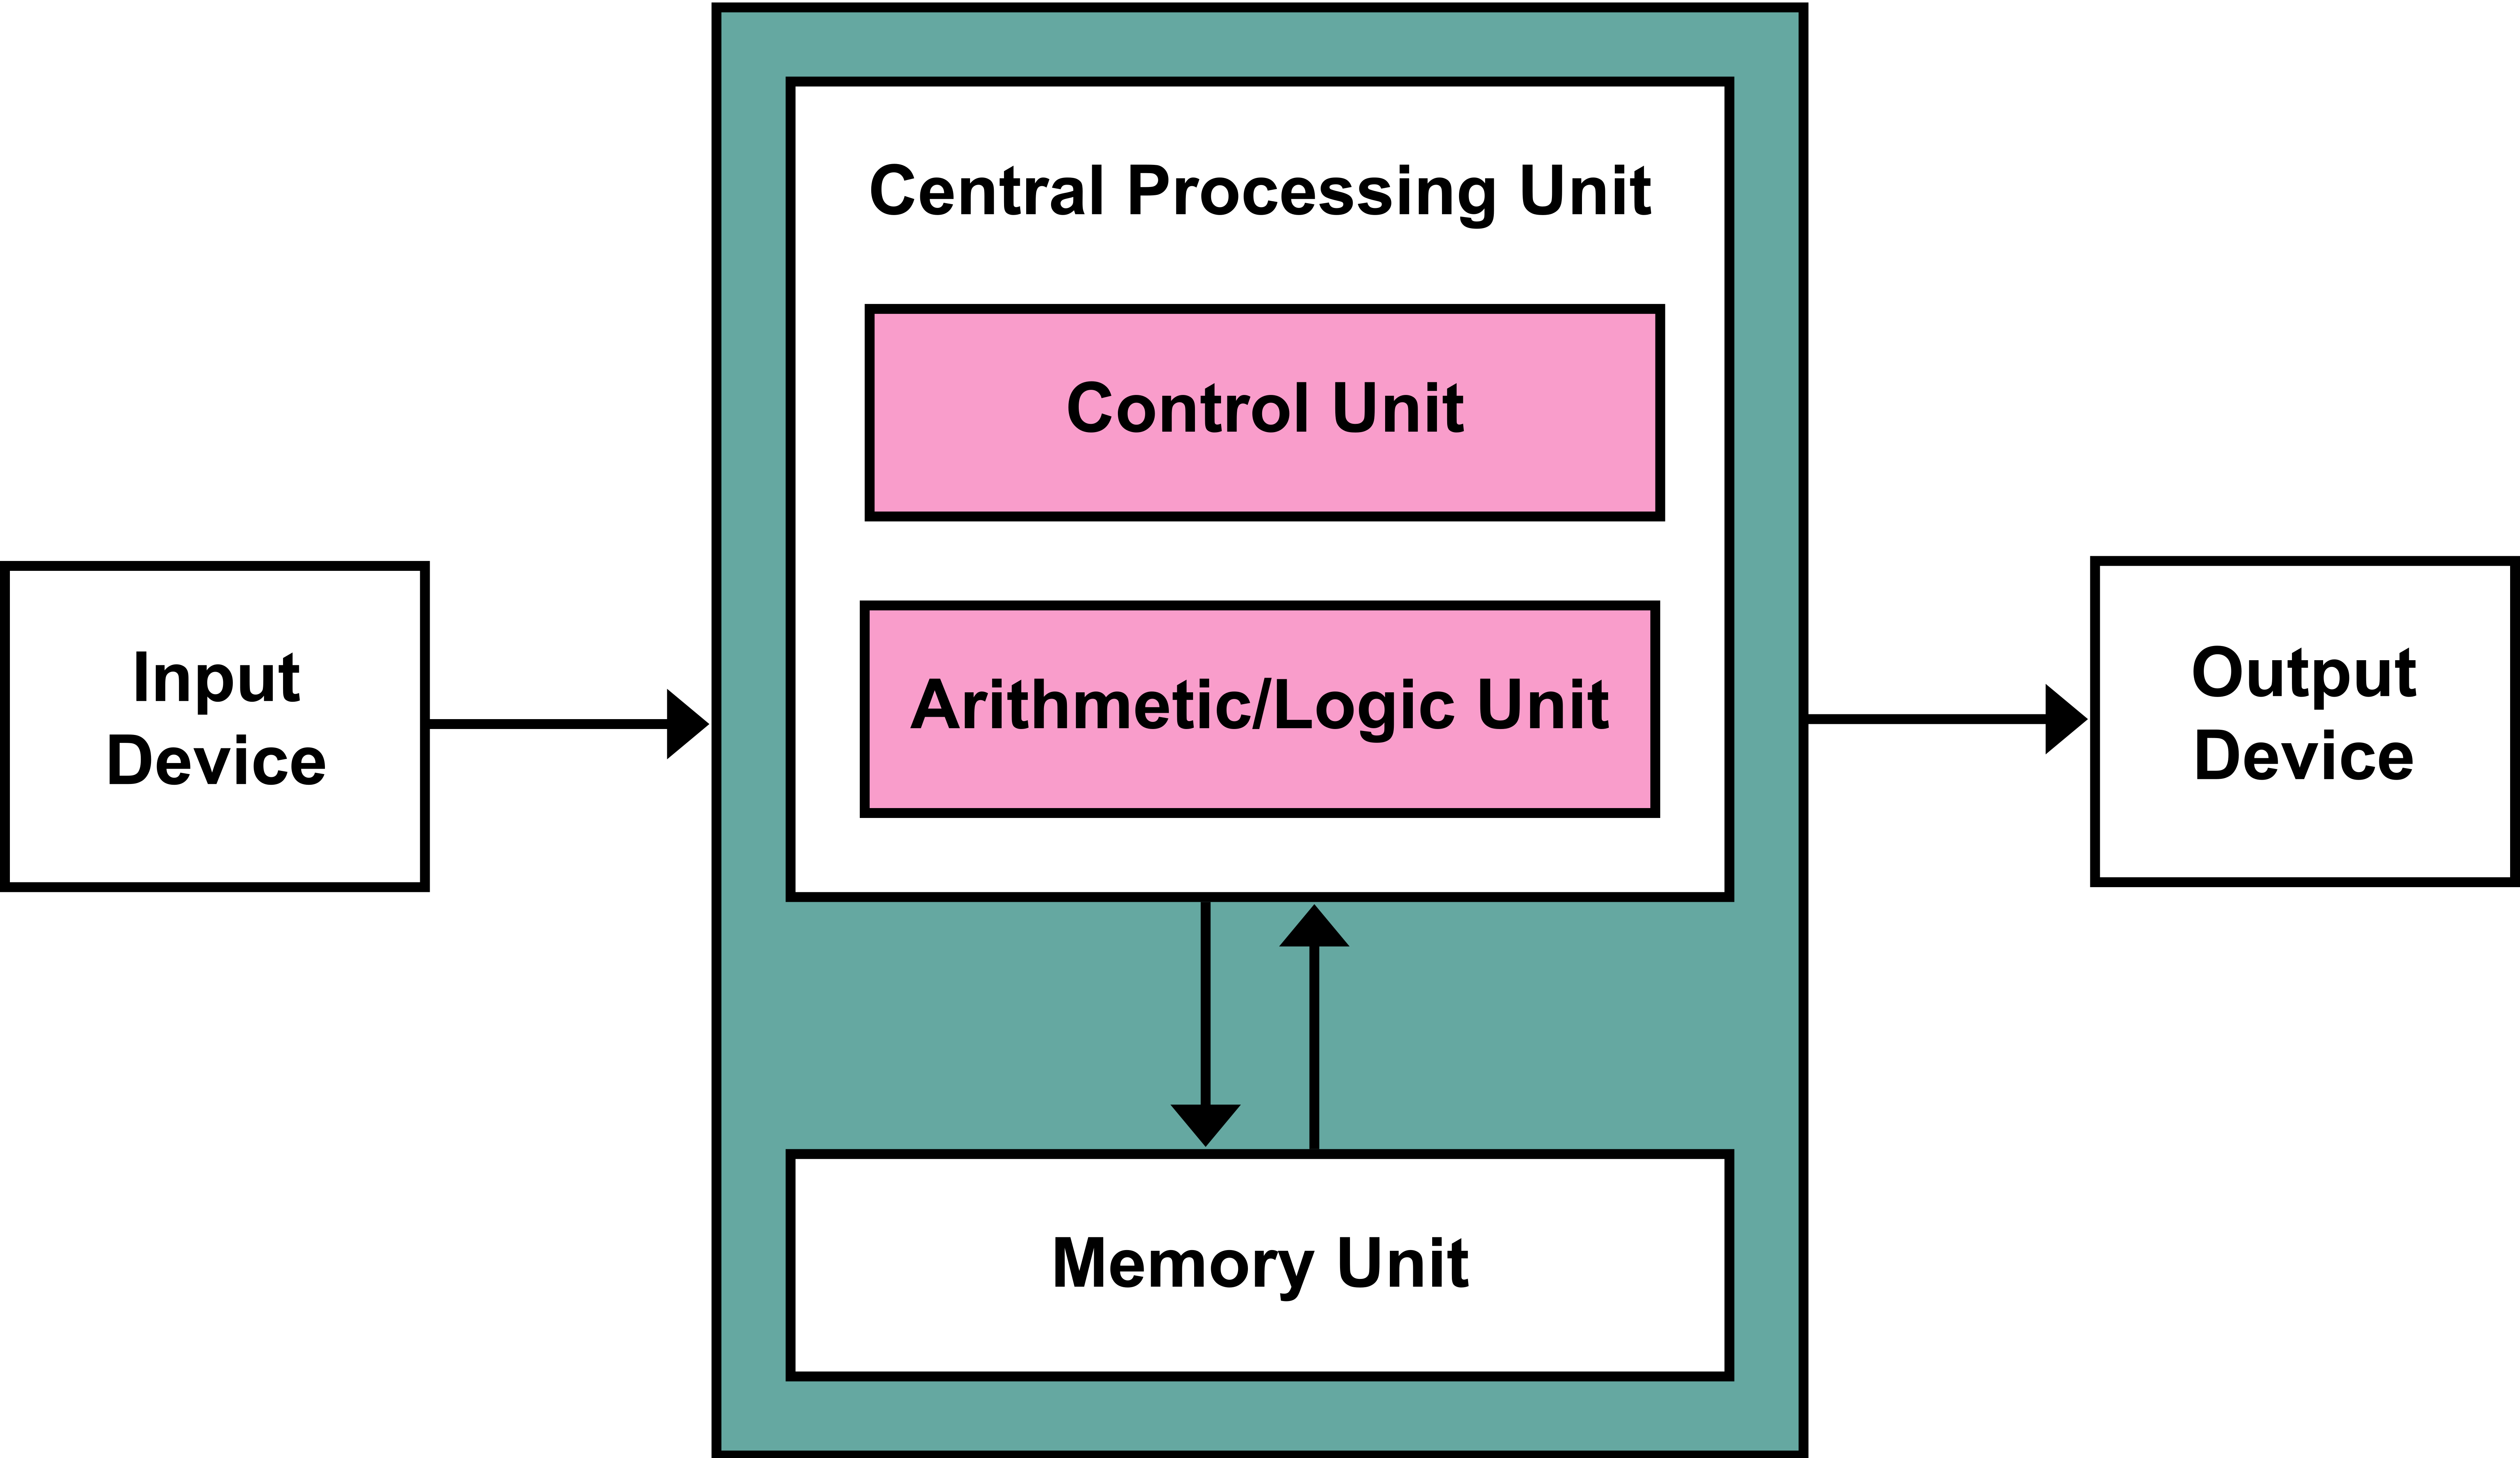
\includegraphics[scale=2]{images/Von_Neumann_Architecture.png}
    \caption{Von Neumann Architecture}
    \label{fig:von_neumann_arch}
\end{figure}

You can also draw figures directly in \LaTeX{} using tikz\footnote{\url{https://texample.net/tikz/}} and some patience. For example, check the source code for Figure~\ref{fig:tikz}, look how nicely it blends with the document (same font, thickness, style).

\begin{figure}[h]
\begin{center}
\begin{tikzpicture}[->,>=stealth',shorten >=1pt,auto,node distance=2.8cm,
                    semithick]
  \tikzstyle{every state}=[fill=red,draw=none,text=white]

  \node[initial,state] (A)                    {$q_a$};
  \node[state]         (B) [above right of=A] {$q_b$};
  \node[state]         (D) [below right of=A] {$q_d$};
  \node[state]         (C) [below right of=B] {$q_c$};
  \node[state]         (E) [below of=D]       {$q_e$};

  \path (A) edge              node {0,1,L} (B)
            edge              node {1,1,R} (C)
        (B) edge [loop above] node {1,1,L} (B)
            edge              node {0,1,L} (C)
        (C) edge              node {0,1,L} (D)
            edge [bend left]  node {1,0,R} (E)
        (D) edge [loop below] node {1,1,R} (D)
            edge              node {0,1,R} (A)
        (E) edge [bend left]  node {1,0,R} (A);
\end{tikzpicture}
\caption{A graph drawn using tikz}
\label{fig:tikz}
\end{center}
\end{figure}

You can draw proof trees as well (but if you have ever taken a logic \& languages elective, you should know this by now).

\[
    \infer[\wedge_r]{\Gamma \vdash A \wedge B}{
        \Gamma \vdash A
        &
        \Gamma \vdash B
    }
\]

You can also write equations, number them, and refer back to them later.

\begin{equation}
\label{eq:euler}
    e^{i\pi} + 1 = 0
\end{equation}

Some claim that Equation~\ref{eq:euler}, also called \emph{Euler's identity}, is one of the most beautiful equations in Mathematics.

The \texttt{listings} package\footnote{\url{https://en.wikibooks.org/wiki/LaTeX/Source_Code_Listings}} provides a nice way for you to include code in your document. It supports a number of programming languages natively, and it is highly customizable. For this document in particular, I left a configuration for Python code. You can see how this is done using the \texttt{lset} command in the \texttt{configs/preamble.tex} file. Check out the final result in the implementation of binary search in Python below:

\begin{lstlisting}
# Iterative Binary Search Function
# It returns index of x in given array arr if present,
# else returns -1
def binary_search(arr, x):
    low = 0
    high = len(arr) - 1
    mid = 0
 
    while low <= high:
        mid = (high + low) // 2

        if arr[mid] < x:
            low = mid + 1
        elif arr[mid] > x:
            high = mid - 1
        else:
            return mid
 
    return -1
\end{lstlisting}